\chapter{Results}\label{Sec:Results}

\section{Maximal Representative Subsample}
 
There is almost always not enough data available to partition it into separate training and test sets without losing significant modelling or testing capability. In these cases, a fair way to properly estimate model prediction performance is to use cross-validation as a powerful general technique[5].

The overly optimistic resubstitution error, is not a good indicator of model performance. To evaluate the actual performance of a model, the given data samples need to be split. The proper procedure uses three sets: training data, validation data, and test data [2]. The holdout method is the most common approach to get a reliable performance estimation: A certain amount of data is reserved for testing while the remainder is used for the actual training. Because the method is very fast, it is useful to use when the algorithm is slow to train and the dataset is large. Training and test sets might not be representative of the same underlying distribution, e.g. class hardly represented in the test set.

 The holdout estimate can be made more reliable by repeating the process with different subsamples. The error rates on the different iterations are averaged to yield an overall error rate. To further reduce the variance of the error estimate, each class is sampled with approximately equal proportions in both datasets, a technique called stratification. Figure X shows the results on the GFI-10 data.

\subsection{Fraction of Positives}

\begin{figure}[ht]
	\begin{center}
		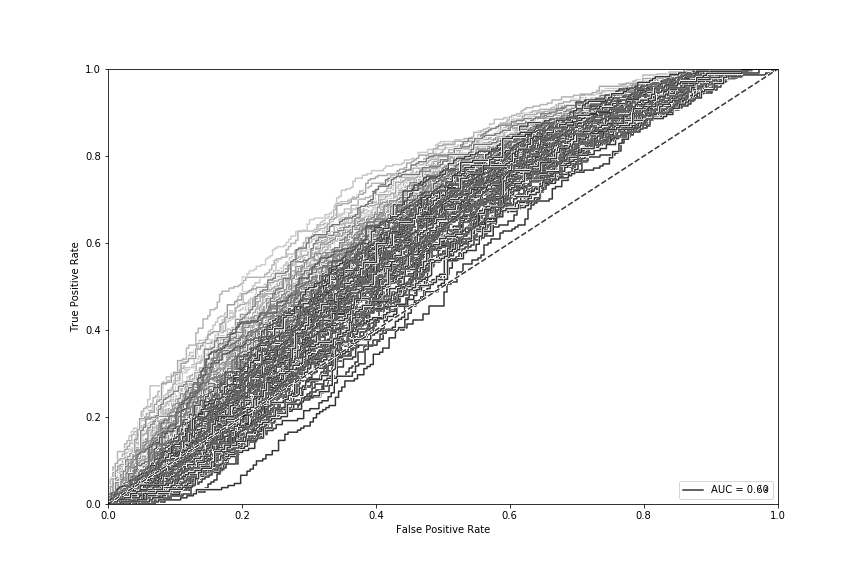
\includegraphics[scale=0.55,angle=0]{fig/Roc_all}
		\label{occ}
		\vspace*{-1.0cm}
		\caption{.}
	\end{center}
\end{figure}

\begin{figure}[ht]
	\begin{center}
		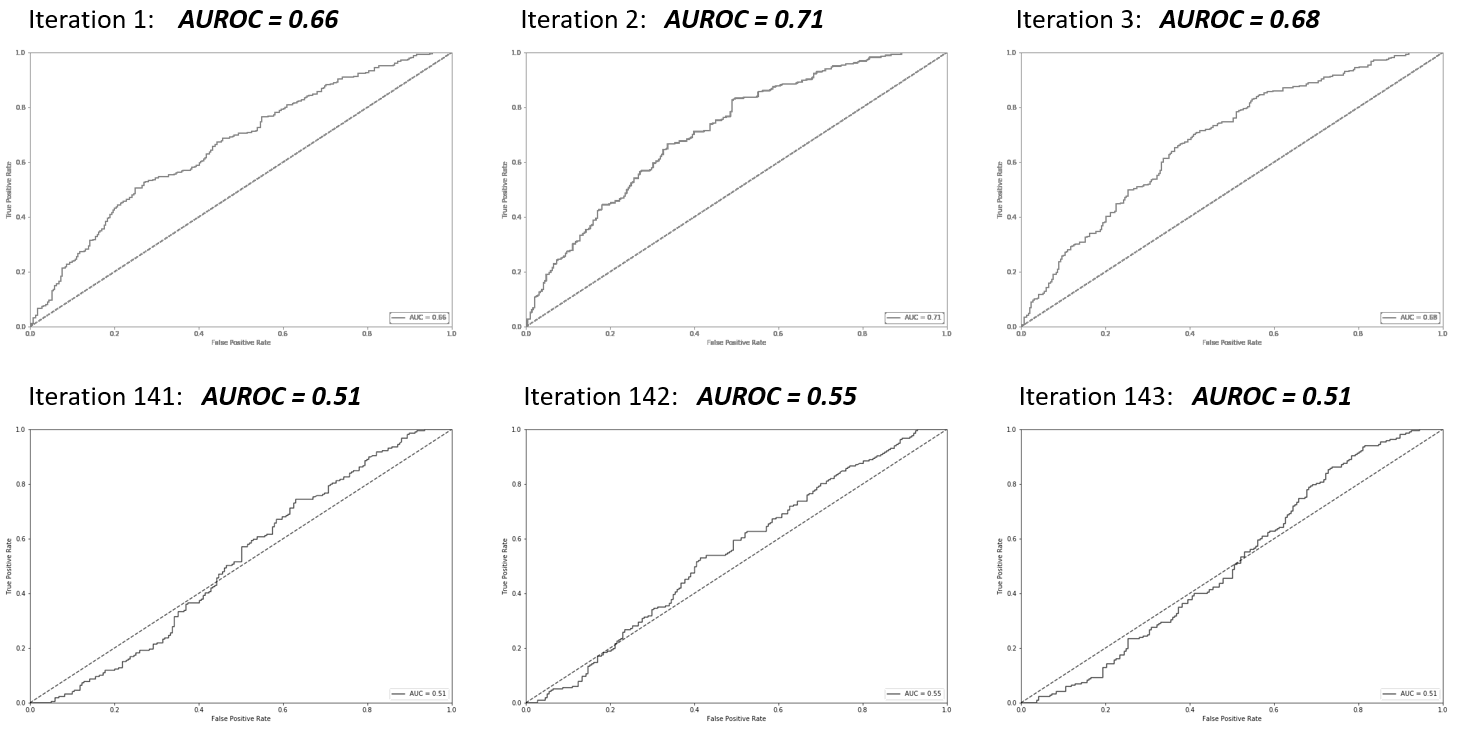
\includegraphics[scale=0.40,angle=0]{fig/Discriminative_Procedure}
		\label{occ}
		\vspace*{-1.0cm}
		\caption{.}
	\end{center}
\end{figure}

Estimating Positive Class Prior with One-Class SVMs. In a simple random sample, one can assume that observations are independent from each other. The complex sample design of GBS however

, e.g. multi-stage samples from different survey periods,
Complex sample design, such as multi-stage samples of schools, classes and students, students from one classroom are likely to be more correlated than those from another classroom. 

we need to compensate for complex survey designs with features including, but not limited to, unequal likelihoods of selection, differences in response rates across key subgroups, and deviations from distributions on critical variables found in the target population from external sources, such as a national Census

\begin{figure}[ht]
	\begin{center}
		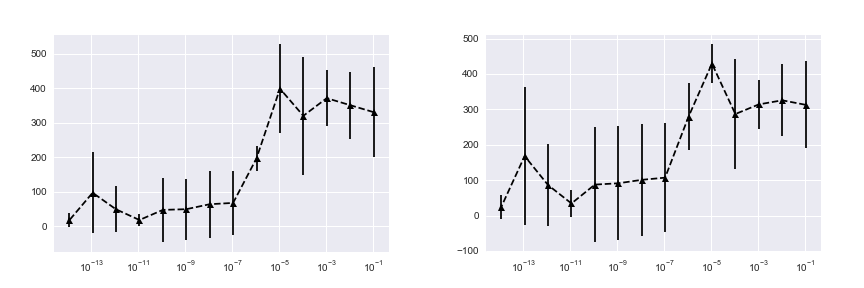
\includegraphics[scale=0.55,angle=0]{fig/occfigure}
		\label{occ}
		\vspace*{-1.0cm}
		\caption{Tuning parameter \(nu\) that controls the trade-off between the fraction of non-representative samples and the number of support vectors in one-class SVM. More than 0.73 of GBS (right) are classified as representative with high confidence (low sdt) for the optimal value \(nu = 10^{-5}\).}
	\end{center}
\end{figure}

\subsection{Evaluation}

most commonly through the development of survey weights for statistical adjustment. If complex sample designs are implemented in data collection but the analysis assumes simple random sampling, the variances of the survey estimates can be underestimated and the confidence interval and test statistics are likely to be biased (Heeringa, West,  Berglund, 2010).

In a recent meta-analysis of 150 sampled research papers analyzing several surveys with complex sampling designs, it is found that analytic errors caused by ignorance or incorrect use of the complex sample design features were frequent. Such analytic errors define an important component of the larger total survey error framework, produce misleading descriptions of populations and ultimately yield misleading inferences (Aurelien, West,  Sakshaug, 2016). It is thus of critical importance to incorporate the complex survey design features in statistical analysis. 


\section{Political Participation and Resilience}

XGBoost is an open-source software library for predictive modelling, created by Tianqi Chen in 2014 [1]. The name XGBoost stands for "Extreme Gradient Boosting" and implements "Gradient Boosting" as proposed in Greedy Function Approximation: A Gradient Boosting Machine by Friedman, while the term "extreme" refers to the engineering goal to maximize the resources used by the algorithm to achieve high accuracy, computational efficiency and scalability. What started off as a terminal application for a research project, has become a scalable end-to-end tree boosting system that has integrations with scikit-learn in Python, the caret package in R, as well as big data frameworks like Apache Spark and Hadoop. Since its introduction, XGBoost has been used in more than half of the winning solutions in Kaggle competitions, after it gained much popularity and attention in the community by winning the Higgs boson machine learning challenge.
